\section{Symmetric Monoidal Bicategories}
\label{sec:constr-symm-mono}

In this section we will discuss how the functor $\mathcal{H}$ from the previous section extends to a functor from the iconic tricategories of monoidal double categories, braided monoidal double categories, and symmetric monoidal double categories, which we will denote with ${\mathcal{M}on\mathcal{D}bl^f_g}$, ${\mathcal{B}r\mathcal{M}on\mathcal{D}bl^f_g}$, and ${\mathcal{S}ym\mathcal{M}on\mathcal{D}bl^f_g}$, respectively. Their images are the iconic tricategories  of monoidal bicategories, braided monoidal bicategories, and symmetric monoidal bicategories, $\mathcal{M}on\mathcal{B}icat$, $\mathcal{B}r\mathcal{M}on\mathcal{B}icat$, and $\mathcal{S}ym\mathcal{M}on\mathcal{B}icat$, respectively.

Note that there are several related notions of each of these tricategories, depending on whether we want the functors within these tricategories to be lax monoidal, oplax monoidal, or strongly monoidal. We represent these versions with a subscript $ l,p,$ or $c$, respectively. 
As we have observed before, we restrict to transformations in $\mathcal{D}bl$ that are horizontally strong. Under this condition, we will prove the main theorem of this section, stated below. %We leave a further generalization to future work.    
%[{\it this seems out of context now..}]

\begin{thm}\label{thm:trifunctor2}
For $w=l,p,$ or $c$, the functor $\mathcal{H}: \mathcal{D}bl^f_g \rightarrow \mathcal{B}icat$ extends to functors 
\begin{align}
\mathcal{H}^M_w: \hspace{1cm} &{\mathcal{M}on\mathcal{D}bl^f_g}_w &\rightarrow \hspace{1cm} &{\mathcal{M}on\mathcal{B}icat}_w\\
\mathcal{H}^{B}_w: \hspace{1cm} &{\mathcal{B}r\mathcal{M}on \mathcal{D}bl^f_g}_w &\rightarrow \hspace{1cm} &{\mathcal{B}r\mathcal{M}on\mathcal{B}icat}_w\\ 
 \mathcal{H}^{S}_w: \hspace{1cm} &{\mathcal{S}ym\mathcal{M}on\mathcal{D}bl^f_g}_w &\rightarrow \hspace{1cm} &{\mathcal{S}ym \mathcal{M}on\mathcal{B}icat}_w
\end{align} 
\end{thm}


  
 \begin{lem}
  Let ${\bf S,T}$ be iconic tricategories with products. Any iconic trifunctor $\mathcal{T}: T \rightarrow S$ that preserves products, preserves  monoidal objects, 1-cells and 2-cell as well as any braided or symmetric structure of these objects, 1-cells and 2-cells.
 \end{lem}
 
 \begin{proof}
Let $A$ be a monoidal object. The functor $\mathcal{T}$ preserves products, so we have a product $\cT(A) \times_{\cT} \cT(A) = \cT(A \times A)$. As a consequence $\ten\maps
  A\times A\to A$ induces a 1-cell $\ten_{\mathcal{T}} \maps
 \mathcal{T}A\times_{\cT} \mathcal{T} A\to\mathcal{T}A$ with a unit 1-cell $I_{\mathcal{T}}$, where $\cT(f) \ten_{\cT} \cT(g) := \cT(f \ten g)$ and $I_{\cT}:= \mathcal{T}(I)$. 
 
 Note that conditions $(iii)$ and $(iv)$ of definition \ref{def:Iconfunc} imply that for all 1-cells $f,g$ we have the equality $\cT(f \odot g) = \cT(f) \odot \cT(g)$ and for the identity 1-cell $\id_A$, $\cT(\id_A) = \id_{\cT(A)}$. Hence, the associativity 2-cell of $A$ gives rise to a 2-cell
  \[\vcenter{\xymatrix@C=6pc{\cT(A)\times\cT(A)\times\cT(A) \rtwocell^{\ten_{\cT}
        (\Id\times\ten_{\cT})}_{\ten_{\cT}(\ten_{\cT}\times\Id)}{\hspace{.2cm}\fa_{\cT}\eqv} &\cT(A) }}\]
  which simply equals $\cT(\alpha)$.
  
  Likewise, the unit constraints $l, r$ as well as the constraints for (braided) monoidal 1-cells $\sigma$ induce 1-cells $l_{\cT}, r_{\cT}$, and $\sigma_{\cT}$, respectively.
  
 Furthermore, the invertible 3-cell filling the Mac Lane pentagon lifts to the invertible 3-cell of the Mac Lane Pentagon for $\cT(A)$. Which is simply its image under $\cT$, composed with the isomorphic $3$-cells given by (iii) of definition \ref{def:Iconfunc}, ensuring that it has the right type.
%   \[\xy
%  (-10,0)*{\ten_{\cT}(\ten_{\cT},\Id)(\ten_{\cT}, \Id, %\Id)}="A";
%  (20,10)*{\ten_{\cT}(\ten_{\cT},\Id)(\Id, \ten_{\cT},\Id)}="B";
%  (50,0)*{\ten_{\cT}(\Id,\ten_{\cT})(\Id, \ten_{\cT},\Id)}="C";
%  (0,-15)*{\ten_{\cT}(\Id, \ten_{\cT})(\ten, \Id, \Id)}="D";
%  (40,-15)*{\ten_{\cT}(\Id, \ten_{\cT})(\Id, \Id, \ten, _{\cT})}="E";
%  (20,-5)*{\scriptstyle\Downarrow \pi \iso};
%  \ar "B";"A";^{\fa_{\cT} \ten_{\cT} \id}
%  \ar "C";"B";^{\fa_{\cT}}
%  \ar "D";"A";_{\fa_{\cT}}
%  \ar "E";"D";_{\fa_{\cT}}
%  \ar "E";"C";^{\id\ten_{\cT} \fa_{\cT}}
%  \endxy
%  \]
  
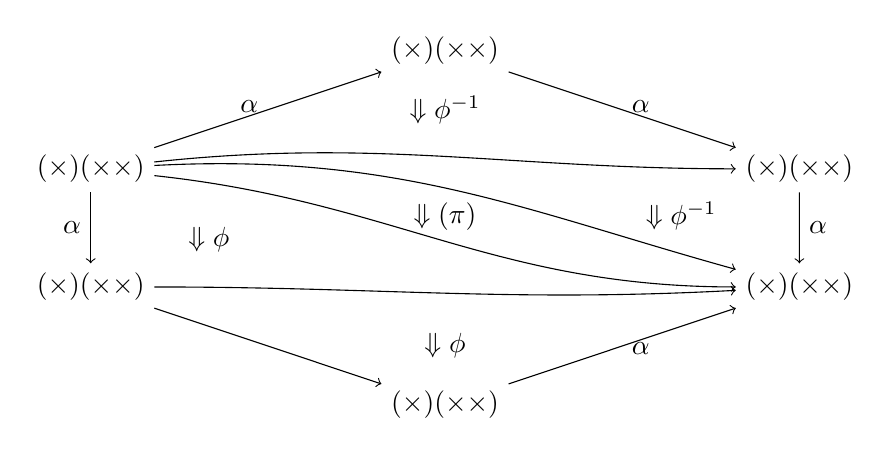
\begin{tikzpicture}[yscale=1.5, xscale=3]
\node(tl) at (0,1) {$\ten (\ten \times \Id)(\ten \times \Id \times \Id)$};
\node(t) at (1.5,2) {$\ten (\ten \times \Id)(\Id \times \ten \times \Id)$};
\node(tr) at (3,1) {$\ten (\Id \times \ten )(\Id \times \ten \times \Id)$};
\node(br) at (3,0) {$\ten (\Id \times \ten )(\Id \times \Id \times \ten )$};
\node(b) at (1.5,-1) {$\ten (\ten \times \Id)(\Id \times \Id \times \ten )$};
\node(bl) at (0,0) {$\ten (\Id \times \ten )(\ten \times \Id \times \Id)$};
\draw[->] (tl) to node[left, yshift=1pt] {$\alpha \ten \id$} (t);
\draw[->] (t) to node[right, yshift=1pt] {$\alpha$} (tr);
\draw[->] (tr) to node[right] {$\id \ten \alpha$} (br);
\draw[->] (tl) to node[left] {$\alpha$} (bl);
\draw[->] (bl) to node[left,yshift=-1pt] {$\id$} (b);
\draw[->] (b) to node[right,yshift=-1pt] {$\alpha$} (br);
\draw[->] (tl) to [in=155, out=5] (br);
\draw[->] (tl) to [in=180, out=-10] (br);
\draw[->] (tl) to [in=180, out=10](tr);
\draw[->] (bl) to [in=185, out=0](br);
\node at (1.5,.6) {$\Downarrow \cT(\pi) \iso$};
\node at (2.5,.6) {$\Downarrow \phi^{-1} \iso$};
\node at (1.5,1.5) {$\Downarrow \phi^{-1} \iso$};
\node at (.5,.4) {$\Downarrow \phi \iso$};
\node at (1.5,-.5) {$\Downarrow \phi \iso $};
\end{tikzpicture}  

 Note that there may be several way to past these 3-cells, but by coherence of pseudofunctors, the result is the same. Likewise, the isomorphic 3-cells $\mu, \lambda,\rho$ and the isomorphic 3-cells $R,S$, and $v$ witnessing the braiding and syllepsis, lift to the appropriate 3-cell for $\cT(A)$. This is also the case for the isomorphic 3-cells $R,S$ that characterise the braiding. 
   Finally, we need to show that the three equations between pasting composites of $\pi_{\cT}, \mu_{\cT}, \lambda_{\cT}, \rho_{\cT}$ hold ???

The argument for 1-cells and 2-cells is similar. 
Let $f,g:A \rightarrow B$ be monoidal 1-cells and let $\alpha: f \Rightarrow g$ be a monoidal 2-cell.
The 2-cells $\chi: \otimes_B \odot (f,f) \Rightarrow f \odot \otimes_A$ and $\iota: I_B \Rightarrow f \odot I_A$ are mapped to $\cT(\chi): \otimes_{\cT(B)} \odot (\cT(f),\cT(f)) \Rightarrow \cT(f) \odot \otimes_{\cT(A)}$ and $\iota: I_{\cT(B)} \Rightarrow \cT(f) \odot I_{\cT(A)}$. Similarly, any 2-cell witnessing a braiding $u: \sigma_B \odot \chi  \Rightarrow \chi \odot f\sigma_A$  is mapped to $\cT(u): \sigma_{\cT(B)} \odot \cT(\chi)  \Rightarrow \cT(\chi) \odot \cT(f)\sigma_{\cT(A)}$.
Analogously to $\alpha$, the invertible 3-cells $\omega, \gamma$, and $\delta$, and $\Pi$ and $M$ are lifted to their images under $\cT$, augmented with instances of $\phi$ to ensure that the 3-cells have the right type.
 It is left to show that the equations pasting composites of these 3-cells together commute.
 \end{proof}
 

\subsection{Lifting Symmetric Monoidal Structures}
We are now ready to lift monoidal structures from double categories to
bicategories.  If we had a theory of symmetric monoidal tricategories,
we could do this by improving \autoref{thm:h-functor} to say that
$\cH$ is a symmetric monoidal functor, and then conclude that it
preserves pseudomonoids.  However, in the absence of such a theory, we
give a direct proof.

\begin{rmk}\label{rmk:sym}
  For monoidal bicategories, there is a notion in between braided and
  symmetric, called \emph{sylleptic}, in which the the braiding is
  self-inverse up to an isomorphism (the \emph{syllepsis}) but this
  isomorphism is not maximally coherent.  Since in our approach the
  syllepsis will be an isomorphism of the form
  $\theta_{\fhat,\fhat'}$, it is \emph{always} maximally coherent;
  thus our method cannot produce sylleptic monoidal bicategories that
  are not symmetric.
\end{rmk}

\begin{lem}\label{thm:mon11-monbi}
  If \lD\ is a {\bf fibrant monoidal double category}, then $\cH(\lD)$ is a
  monoidal bicategory.  
\end{lem}


\begin{proof}[Proof of \autoref{thm:mon11-monbi}]
  A monoidal bicategory is defined to be a tricategory with one
  object.  We use the definition of tricategory
  from~\cite{nick:tricats}, which is the same as that
  of~\cite{gps:tricats} except that the associativity and unit
  constraints are pseudo natural adjoint equivalences, rather than
  merely pseudo transformations whose components are equivalences.

  The functor \cH\ evidently preserves products, so $\ten\maps
  \lD\times\lD\to\lD$ induces a functor $\ten\maps
  \cH(\lD)\times\cH(\lD)\to \cH(\lD)$, and of course $I$ is still the
  unit.  The associativity constraint of \lD\ is a natural isomorphism
  \[\vcenter{\xymatrix@C=5pc{\lD\times\lD\times\lD \rtwocell^{\ten
        (\Id\times\ten)}_{\ten(\ten\times\Id)}{\fa\iso} &\lD }}\]
  so by \autoref{thm:h-locfr} it gives rise to a pseudo natural
  adjoint equivalence
  \[\vcenter{\xymatrix@C=6pc{\cH(\lD)\times\cH(\lD)\times\cH(\lD) \rtwocell^{\ten
        (\Id\times\ten)}_{\ten(\ten\times\Id)}{\fahat\eqv} &\cH(\lD) }}\]
  Likewise, the unit constraints of \lD\ induce pseudo natural adjoint
  equivalences.

  The final four pieces of data for a monoidal bicategory are
  invertible modifications relating various composites of the
  associativity and unit transformations.  The first is a
  ``pentagonator'' which relates the two ways to go around the Mac
  Lane pentagon:
  \[\xy
  (-10,0)*{((A\ten B)\ten C)\ten D}="A";
  (20,10)*{(A\ten (B\ten C))\ten D}="B";
  (50,0)*{A\ten ((B\ten C)\ten D)}="C";
  (0,-15)*{(A\ten B)\ten (C\ten D)}="D";
  (40,-15)*{A\ten (B\ten (C\ten D))}="E";
  (20,-5)*{\scriptstyle\pi\Downarrow\iso};
  \ar "B";"A";^{\fahat\ten U_D}
  \ar "C";"B";^{\fahat}
  \ar "D";"A";_{\fahat}
  \ar "E";"D";_{\fahat}
  \ar "E";"C";^{U_A\ten \fahat}
  \endxy
  \]
By Lemma's ~\ref{thm:comp-unit},  ~\ref{thm:comp-compose}, and ~\ref{thm:comp-ten}, the outside of this diagram commutes.  
 As a result, we can construct $\pi$ by Lemma \ref{lem:modification}. The other invertible modifications $\mu, \lambda$, and $\rho$ are constructed in the same way.

  Finally, we must show that three equations between pasting
  composites of 2-cells hold, relating composites of
  $\pi,\mu,\lambda,\rho$.  However, in each of these equations, both
  the domain and the codomain of the 2-cells involved are companions
  of the same isomorphism in $\lD_0$.  For the 5-associahedron, this
  isomorphism is the unique constraint
  \[(((A\ten B)\ten C)\ten D)\ten E \too[\iso] A\ten (B\ten (C\ten
  (D\ten E)));
  \]
  for the other two it is simply the associator $(A\ten B)\ten C
  \too[\iso] A\ten (B\ten C)$.  By Lemma \ref{lem:modification},
  every 2-cell in these diagrams is a $\theta$-isomorphism relating
  two companions of the same vertical isomorphism.  Therefore, Lemma ~\ref{lem:equal} implies that the three equations hold.
\end{proof}


  Now suppose that \lD\ is braided; to show that $\cH(\lD)$ is braided
  we seemingly must first have a definition of braided monoidal
  bicategory.  The interested reader may follow the tortuous path of
  the definition of braided monoidal 2-categories and bicategories
  through the literature, starting from~\cite{kv:2cat-zam,kv:bm2cat}
  and continuing, with occasional corrections,
  through~\cite{bn:hda-i,ds:monbi-hopfagbd,crans:centers,mccrudden:bal-coalgb},
  and~\cite{gurski:brmonbicat}.  However, the details of the
  definition are essentially unimportant for us; since our constraints
  and coherence are produced in a universal way, any reasonable data
  can be produced and any reasonable axioms will be satisfied.  For
  concreteness, we use the definition of~\cite{mccrudden:bal-coalgb}.

\begin{lem}\label{thm:br11-brbi}
  If \lD\ is a {\bf fibrant braided monoidal double category}, then $\cH(\lD)$ is a
 braided monoidal bicategory.  
\end{lem}

\begin{proof}
  The first piece of data we require to make $\cH(\lD)$ braided is a
  pseudo natural adjoint equivalence $\mathord{\otimes} \too[\eqv]
  \mathord{\otimes}\circ \tau$, where $\tau$ is the switch
  isomorphism.  This arises by \autoref{thm:h-locfr} from the braiding $\sigma$
  of \lD.  We also require two invertible modifications filling the
  usual hexagons for a braiding:
  \begin{equation}
  \begin{aligned}
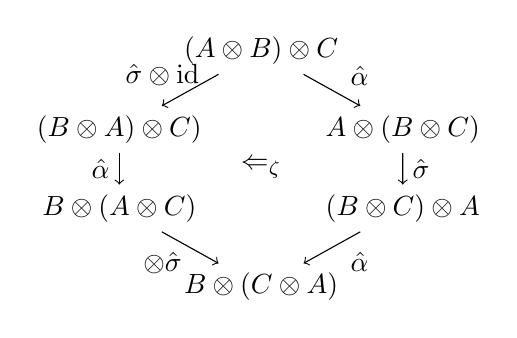
\begin{tikzpicture}[xscale=0.9]
\node (t) at (2,3) {$(A \otimes B) \otimes C$};
\node (tl) at (0,2) {$(B \otimes A) \otimes C)$};
\node (bl) at (0,1) {$B \otimes  (A \otimes C)$};
\node (b) at (2,0) {$B \otimes (C \otimes A)$};
\node (tr) at (4,2) {$A \otimes (B \otimes C)$};
\node (br) at (4,1) {$(B \otimes C) \otimes A$};
\draw[->] (t) to node [above,xshift=10pt, yshift=-2] {$\hat{\alpha}$} (tr);
\draw[->] (tr) to node [right] {$\hat{\sigma}$} (br);
\draw[->] (br) to node [below,xshift=10pt, yshift=2pt] {$\hat{\alpha}$} (b);
\draw[->] (t) to node [above,xshift=-10pt, yshift=-2pt] {$\hat{\sigma} \otimes \mbox{id}$} (tl);
\draw[->] (tl) to node [left] {$\hat{\alpha}$} (bl);
\draw[->] (bl) to node [below,xshift=-10pt,yshift=2pt] {$\mathid \otimes \hat{\sigma}$} (b);
\node at (2,1.5) {$\Leftarrow_{\zeta \iso}$};
\end{tikzpicture}
  \end{aligned}
\hspace{5pt}\mbox{and} \hspace{5pt}
\begin{aligned}
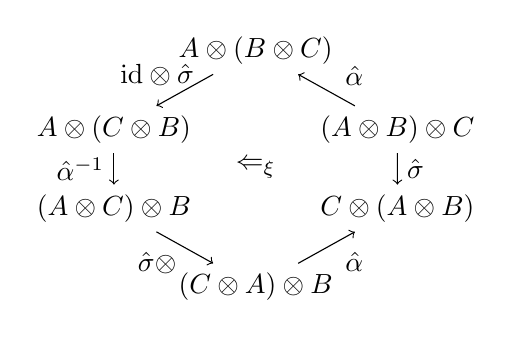
\begin{tikzpicture}[xscale=0.9]
\node (t) at (2,3) {$A \otimes (B \otimes C)$};
\node (tl) at (0,2) {$A \otimes (C \otimes B)$};
\node (bl) at (0,1) {$(A \otimes  C) \otimes B$};
\node (b) at (2,0) {$(C \otimes A) \otimes B$};
\node (tr) at (4,2) {$(A \otimes B) \otimes C$};
\node (br) at (4,1) {$C \otimes (A \otimes B)$};
\draw[->] (tr) to node [above,xshift=10pt, yshift=-2] {$\hat{\alpha}$} (t);
\draw[->] (tr) to node [right] {$\hat{\sigma} $} (br);
\draw[->] (b) to node [below,xshift=10pt, yshift=2pt] {$\hat{\alpha}$} (br);
\draw[->] (t) to node [above,xshift=-10pt, yshift=-2pt] {$\mbox{id} \otimes \hat{\sigma}$} (tl);
\draw[->] (tl) to node [left] {$\hat{\alpha}^{-1}$} (bl);
\draw[->] (bl) to node [below,xshift=-10pt,yshift=2pt] {$\hat{\sigma} \otimes \mathid$} (b);
\node at (2,1.5) {$\Leftarrow_{\xi \iso}$};
\end{tikzpicture}
\end{aligned}
\end{equation}

  As before, since the corresponding hexagons commute in $\lD_0$, by Lemma ~\ref{lem:modification} we have $\theta$-isomorphisms that we can take as $\ze$
  and $\xi$.  Finally, we must verify that the four 2-cell diagrams
  in~\cite[p136--139]{mccrudden:bal-coalgb} involving \ze\ and \xi\
  commute.  As with the axioms for a monoidal bicategory, both sides
  of these equalities are made up of $\theta$s relating companions of
  a single morphism in $\lD_0$, and thus by uniqueness they must be
  equal.

%   for a Gray monoid these can be
%   found in~\cite[p216--217]{bn:hda-i}
%   and~\cite[p191--193]{crans:centers}

%   According to~\cite{crans:centers}, there is also a missing unit
%   axiom in the definition of braided Gray monoid
%   in~\cite{bn:hda-i,ds:monbi-hopfagbd}.  In a braided monoidal
%   bicategory, this axiom should become an isomorphism
%   \[\vcenter{\xymatrix{A\ten I \ar[rr] \ar[dr] &
%       \ar@{}[d]|-{\Downarrow\iso}& 
%       I\ten A \ar@{<-}[dl]\\ & A}}\]
%   We produce this, and its coherence, in the same way.
\end{proof}

\begin{lem}\label{thm:sym11-symbi}
  If \lD\ is a {\bf fibrant symmetric monoidal double category}, then $\cH(\lD)$ is a
 symmetric monoidal bicategory.  
\end{lem}

\begin{proof}
Suppose that \lD\ is symmetric.  To make $\cH(\lD)$ symmetric,
  we require first a \emph{syllepsis}, i.e.\ an invertible
  modification
  \[
 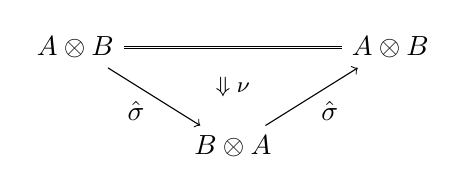
\begin{tikzpicture}
 \node (tl) at (-2,1) {$A \otimes B$};
 \node (tr) at (2,1) {$A \otimes B$};
 \node (b) at (0,-.25) {$B \otimes A$};
 \draw[double] (tl)  -- (tr);
 \draw[->] (tl) to node[left, yshift=-5pt]{$\hat{\sigma}$} (b);
 \draw[->] (b) to node[right, yshift=-5pt] {$\hat{\sigma}$}(tr);
 \node at (0,0.5) {\footnotesize $\Downarrow \nu\iso$}; 
 \end{tikzpicture}
 \]
  Since the braiding in $\lD_0$ is self-inverse, the top and bottom of
  this triangle are both companions of $1_{A\ten B}$; thus we have a
  $\theta$-isomorphism between them which we take as $\nu$.  For
  $\cH(\lD)$ to be sylleptic, the syllepsis must satisfy the two
  axioms on~\cite[p144--145]{mccrudden:bal-coalgb}.  As before, these
  diagrams of 2-cells are made up entirely of $\theta$s relating
  companions of a single morphism in $\lD_0$, so they commute by
  uniqueness of $\theta$.

% ; the first two relate
%   companions of associativities and the last two of units.

% .  For a sylleptic Gray monoid, these
%   axioms can be found in~\cite[p128]{ds:monbi-hopfagbd}
%   and~\cite[p207]{crans:centers}; for a sylleptic monoidal bicategory
%   they are in

  Finally, for $\cH(\lD)$ to be symmetric, the syllepsis must satisfy
  one additional axiom, given on~\cite[p91]{mccrudden:bal-coalgb}.
  This follows automatically for the same reasons as before.
%  in~\cite[p131]{ds:monbi-hopfagbd}
%   and~\cite[p208]{crans:centers}.
\end{proof}




\begin{rmk}
  Essentially the same proof as that of \autoref{thm:mon11-monbi}
  shows that any fibrant 2x1-category has an underlying tricategory.
  Note that unlike the construction of bicategories from
  1x1-categories (i.e.\ double categories), this case requires
  fibrancy even in the absence of monoidal structure, since the
  associativity and unit constraints of a 2x1-category are not 1-cells
  but rather morphisms of 0-cells.  There are many naturally occurring
  fibrant symmetric monoidal 2x1-categories, such as $\lD_0=$
  commutative rings, $\lD_1=$ algebras, and $\lD_2=$ modules, or the
  symmetric monoidal 2x1-category of \emph{conformal nets} defined
  in~\cite{bdh:confnets-i}.  All of these have underlying
  tricategories, which will be symmetric monoidal for any reasonable
  definition of symmetric monoidal tricategory.  More generally, as
  stated in \S\ref{sec:introduction}, we expect any fibrant $(n\times
  k)$-category to have an underlying $(n+k)$-category.
\end{rmk}

Now we will show that the functor $\cH$ lifts monoidal double functors to monoidal pseudo functors. We use definition 3.3.1 of ~\cite{nick:tricats} of a trifunctor, between tricategories with one object. From now on we will assume that all double categories are fibrant.

\begin{lem}\label{lem:monfun}
If $F$ is a {\bf strong monoidal double functor}, $\cH(F)$ is a monoidal pseudo functor, if $F$ is {\bf lax monoidal double functor}, $\cH(F)$ is a lax monoidal pseudo functor, and if $F$ is an {\bf oplax monoidal double functor}, $\cH(F)$ is an oplax monoidal pseudo functor. 
\end{lem}

\begin{proof}
Let $\D, \E$ be monoidal double categories, and let $F:\D \rightarrow \E$ be a strong monoidal double functor. 
By Theorem ~\ref{thm:h-locfr}, the vertical transformations $\phi: \otimes \circ (F,F) \rightarrow F \circ \otimes $ and $\phi_u: I_{\E} \rightarrow F(I_{\D})$, are mapped by $\cH$ to the pseudo natural adjoint equivalences $\hat{\phi}$ and $\hat{\phi_u}$.

We need to show that there exist invertible modifications relating  different compositions of $F$, $\hat{\phi}$, $\hat{\phi_u}$, the associator, and the unitors. 
The components of the first one of these modifications are given below.

\begin{equation}
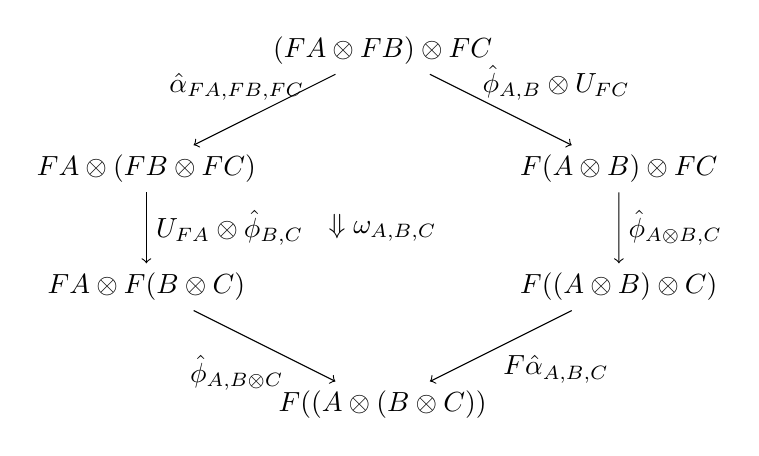
\begin{tikzpicture}[scale=1.5]
\node (t) at (2,3) {$(FA \otimes FB) \otimes FC$};
\node (tl) at (0,2) {$FA \otimes (FB \otimes FC)$};
\node (bl) at (0,1) {$FA \otimes  F(B \otimes C)$};
\node (b) at (2,0) {$F((A \otimes (B \otimes C))$};
\node (tr) at (4,2) {$F(A \otimes B) \otimes FC$};
\node (br) at (4,1) {$F((A \otimes B) \otimes C)$};
\draw[->] (t) to node [above,xshift=20pt] {$\hat{\phi}_{A,B} \otimes U_{FC}$} (tr);
\draw[->] (tr) to node [right] {$\hat{\phi}_{A \otimes B,C} $} (br);
\draw[->] (br) to node [below,xshift=20pt] {$F\hat{\alpha}_{A,B,C}$} (b);
\draw[->] (t) to node [above,xshift=-10pt] {$\hat{\alpha}_{FA, FB, FC}$} (tl);
\draw[->] (tl) to node [right] {$U_{FA} \otimes \hat{\phi}_{B,C} $} (bl);
\draw[->] (bl) to node [below,xshift=-10pt] {$\hat{\phi}_{A, B \otimes C}$} (b);
\node at (2,1.5) {$\Downarrow \omega_{A,B,C}$};
\end{tikzpicture}
\end{equation} 

By Lemmas ~\ref{thm:comp-unit}
and ~\ref{thm:comp-ten}, the morphisms above are companions first coherence diagram for monoidal functors. As a result, the existence of $\omega$ follows from Lemma \ref{lem:modification}. The other modifications, $\delta$ and $\gamma$, are constructed in the same way.

Finally, we need to show that the equalities between compositions of structure modifications hold, as described in definition 3.3.1 of ~\cite{nick:tricats}. The source and target of these composites are $F(((A \otimes B) \otimes C) \otimes D) \rightarrow FA \otimes ( FB \otimes (FC \otimes FD)))$, and $F(A \otimes B) \rightarrow F(A \otimes (I \otimes B))$, respectively.  Each individual composed 2-cell is a $\theta$-isomorphism, either by definition, or by Lemma \ref{thm:theta-nat}. As a result, the equality follows from uniqueness of compositions of $\theta$-isomorphisms.

By the same argument, one can show that oplax/lax monoidal double functors are lifted by $\mathcal{H}$ to lax/oplax monoidal pseudofunctors. In the latter case, the arrows corresponding to all instances of $\phi$ are reversed. 
\end{proof}


\begin{lem}\label{lem:brfun}
Let $(F, \phi) :\D \rightarrow \E$ be a {\bf braided monoidal double functor}, then $\cH(F):\cH(\D) \rightarrow \cH(\E)$ is a braided monoidal pseudofunctor. 
\end{lem}

\begin{proof}
We follow the definition of a braided monoidal pseudo functor given in ~\cite{mccrudden:bal-coalgb}.
We need to show that there exists an invertible modification with the following components:

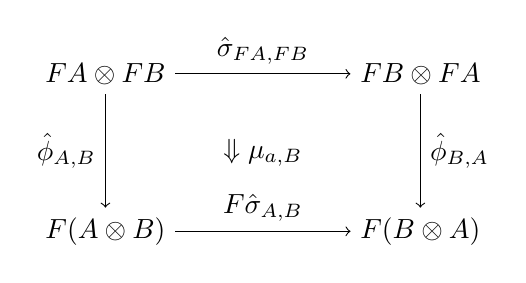
\begin{tikzpicture}[xscale=4,yscale=2]
\node (tl) at (0,1) {$FA \otimes FB$};
\node (tr) at (1,1) {$FB \otimes FA$};
\node (bl) at (0,0) {$F(A \otimes B)$};
\node (br) at (1,0) {$F(B \otimes A)$};
\node at (0.5,0.5){$\Downarrow \mu_{a,B}$};
\draw[->] (tl) to node [above]{$\hat{\sigma}_{FA,FB}$} (tr);
\draw[->] (bl) to node [above]{$F\hat{\sigma}_{A,B}$} (br);
\draw[->](tl) to node [left]{$\hat{\phi}_{A,B}$} (bl);
\draw[->] (tr) to node [right]{$\hat{\phi}_{B,A}$} (br);
\end{tikzpicture}
 
As before, this modification is induced by the characteristic diagram for braided monoidal functors, by Lemma ~\ref{lem:modification}.
It remains to show that the two diagrams of 2-cells given  in ~\cite{mccrudden:bal-coalgb} commute. The domain and codomain of these compositions are of the form $(FA \otimes FB) \otimes FC  \rightarrow F(B \otimes (C \otimes A))$  and $(FA \otimes FB) \otimes FC) \rightarrow F((C \otimes A) \otimes B)$ in $\E_0$.
Each individual composed 2-cell is a $\theta$-isomorphism, either by definition, or by Lemma ~\ref{thm:theta-nat}. As a result, the equality follows from uniqueness of $\theta$-isomorphisms. 
\end{proof}

\begin{lem}\label{lem:symfun}
Let $F:(\D, \phi) \rightarrow (\E, \phi)$ be a {\bf symmetric monoidal double functor}, then $\cH(F): \cH(\D) \rightarrow \cH(\E)$ is a symmetric monoidal pseudofunctor. 
\end{lem}

Recall that by remark ~\ref{rmk:sym}, any syllepsis obtained by our construction is a $\theta$-isomorphism, which makes it a symmetry. This means that it is sufficient to show that symmetric monoidal double functors are mapped by $\cH$ to sylleptic monoidal pseudo functors. 

Recall that a sylleptic bicategory is a braided bicategory with an additional invertible modification $\nu: \id \rightarrow \hat{\sigma} \odot \hat{\sigma}$. 

Following the definition given in \cite{mccrudden:bal-coalgb}, 
we need to show that the equality between the compositions of 2-cells below holds. 

\begin{equation}
\begin{aligned}
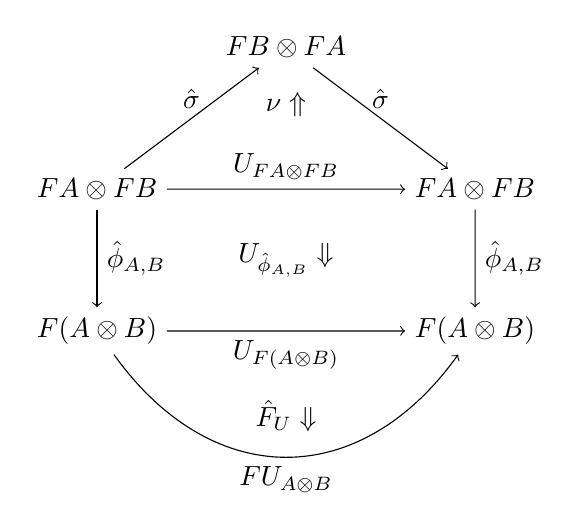
\begin{tikzpicture}[xscale=1.2, yscale=1.8]
\node (t) at (2,3) {$FB \otimes FA$};
\node (tl) at (0,2) {$FA \otimes FB$};
\node (bl) at (0,1) {$F(A\otimes B)$};
\node (tr) at (4,2) {$FA \otimes FB$};
\node (br) at (4,1) {$F(A\otimes B)$};
\draw[->] (t) to node [above] {$\hat{\sigma}$} (tr);
\draw[->] (tr) to node [right] {$\hat{\phi}_{A,B}$} (br);
\draw[->] (tl) to node [above] {$\hat{\sigma}$} (t);
\draw[->] (tl) to node [right] {$\hat{\phi}_{A,B}$} (bl);
\draw[->] (tl) to node [above] {$U_{FA \otimes FB}$} (tr);
\draw[->] (bl) to[in=-135, out=-45] node [below] {$FU_{A\otimes B}$} (br);
\draw[->] (bl) to node [below] {$U_{F(A \otimes B)}$} (br);
\node at (2,2.6) {$\nu \Uparrow$};
\node at (2,1.5) {$U_{\hat{\phi}_{A,B}} \Downarrow$};
\node at (2, 0.4) {$\hat{F}_U \Downarrow$};
\end{tikzpicture}
\end{aligned}
=
\begin{aligned}
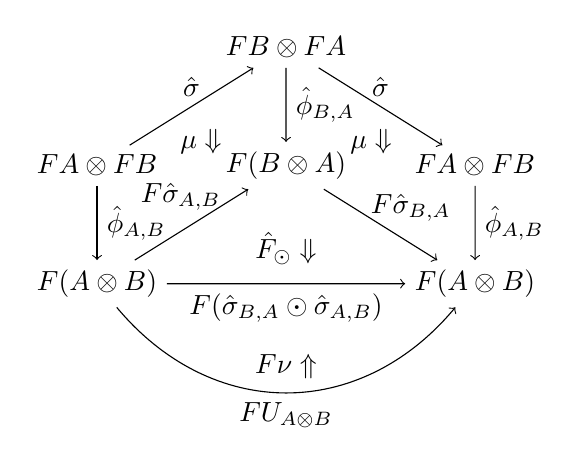
\begin{tikzpicture}[xscale=1.2, yscale=1.5]
\node (t) at (2,3) {$FB \otimes FA$};
\node (tl) at (0,2) {$FA \otimes FB$};
\node (bl) at (0,1) {$F(A\otimes B)$};
\node (m) at (2,2) {$F(B\otimes A)$};
\node (tr) at (4,2) {$FA \otimes FB$};
\node (br) at (4,1) {$F(A\otimes B)$};
\draw[->] (t) to node [above] {$\hat{\sigma}$} (tr);
\draw[->] (t) to node [right] {$\hat{\phi}_{B,A}$} (m);
\draw[->] (tr) to node [right] {$\hat{\phi}_{A,B}$} (br);
\draw[->] (tl) to node [above] {$\hat{\sigma}$} (t);
\draw[->] (tl) to node [right] {$\hat{\phi}_{A,B}$} (bl);
\draw[->] (bl) to node [left,yshift=10pt, xshift=14pt] {$F\hat{\sigma}_{A,B}$} (m);
\draw[->] (m) to node [right,xshift=-7,yshift=6] {$F{\hat{\sigma}}_{B,A}$} (br);
\draw[->] (bl) to[in=-135, out=-45] node [below] {$FU_{A\otimes B}$} (br);
\draw[->] (bl) to node [below] {$F({\hat{\sigma}}_{B,A} \odot {\hat{\sigma}}_{A, B})$} (br);
\node at (1.1,2.2) {$\mu \Downarrow$};
\node at (2.9,2.2) {$\mu \Downarrow$};
\node at (2,1.3) {$ \hat{F}_{\odot} \Downarrow$};
\node at (2, 0.3) {$F\nu \Uparrow$};
\end{tikzpicture}
\end{aligned}
\end{equation} 

Each individual 2-cell is a $\theta$-isomorphism. For $U_{\hat{\phi}}$ and $\hat{F}_{\odot}$, 
this follows from Lemma ~\ref{thm:theta-nat}, for $\hat{F}_{U}$ this follows from Lemma ~\ref{lem:FUtheta}, since $\hat{F}_{U}$ equals $F_U$ and for $F \nu$ this follows from Lemma ~\ref{thm:theta-func}. The other 2-cells are $\theta$-isomorphisms by definition.
As a result, we can apply Lemma \ref{lem:equal} to obtain the equality.  

\begin{lem}\label{lem:montran}
Let $\beta: (F, \phi) \rightarrow (G,\psi)$ be a {\bf monoidal vertical transformation}. The image of $\beta$ under $\mathcal{H}$, $\hat{\beta}: (F, \phi) \rightarrow (G,\psi)$, is a monoidal pseudonatural adjoint equivalence.
\end{lem}

\begin{proof}
Following Definition 3 of ~\cite{gg:ldstr-tricat} of a pseudo icon, applied to tricategories with one object, we need to show that there exist invertible modifications $\kappa$ and $\lambda$ of the form:

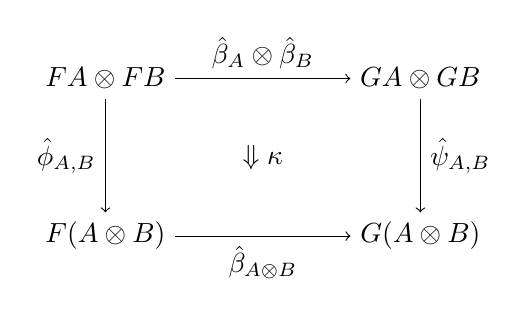
\begin{tikzpicture}[xscale=4, yscale=2]
\node (tl) at (0,1) {$FA \otimes FB$};
\node (bl) at (0,0) {$F(A \otimes B)$};
\node (tr) at (1,1) {$GA \otimes GB$};
\node (br) at (1,0) {$G(A \otimes B)$};
\draw[->] (tl) to node [above] {$\hat{\beta}_A \otimes \hat{\beta}_B$} (tr);
\draw[->] (bl) to node [below] {$\hat{\beta}_{A \otimes B}$} (br);
\draw[->] (tl) to node [left] {$\hat{\phi}_{A,B}$} (bl);
\draw[->] (tr) to node [right] {$\hat{\psi}_{A,B}$} (br);
\node at (0.5,0.5) {$\Downarrow \kappa$};
\end{tikzpicture}
\hspace{1cm}
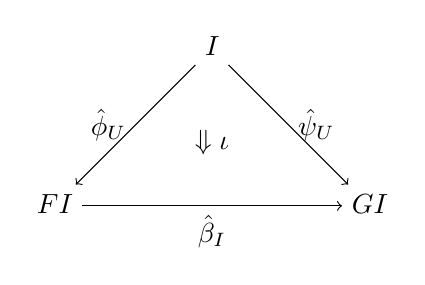
\begin{tikzpicture}[xscale=4,yscale=2]
\node (t) at (0.5,1) {$I_{\E}$};
\node (bl) at (0,0) {$FI_{\D}$};
\node (br) at (1,0) {$GI_{\D}$};
\draw[->] (t) to node [left] {$\hat{\phi}_U$} (bl);
\draw[->] (t) to node [right] {$\hat{\psi}_U$} (br);
\draw[->] (bl) to node [below] {$\hat{\beta}_{I}$} (br);
\node at (0.5,0.4) {$\Downarrow \iota$};
\end{tikzpicture}

This follows from Lemma \ref{lem:modification}. 
It is left to check that the three coherence axioms in definition 3 of ~\cite{gg:ldstr-tricat} hold. These correspond to equalities of compositions of modifications, whose domain and codomain correspond are the isomorphisms $I_{\D} \otimes FA \rightarrow GA$, $FA \otimes I_{\D} \rightarrow GA$, and $(FA \otimes FB) \otimes FC \rightarrow G(A \otimes (B \otimes C))$.
The first of the three equalities is given by the diagrams below.

\begin{equation}
\begin{aligned}
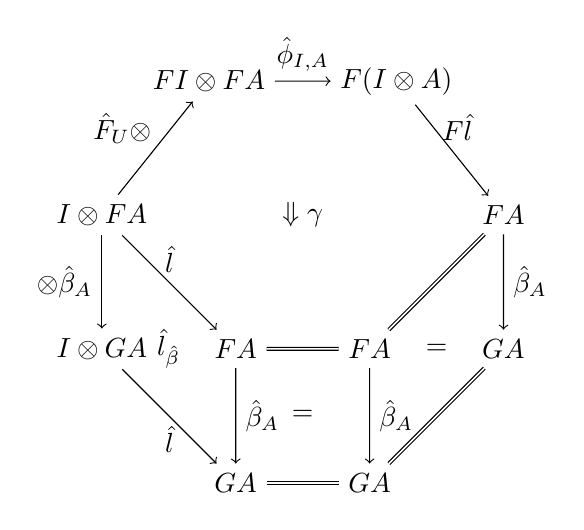
\begin{tikzpicture}[scale=1.7]
\node (llb) at (0,1) {$I \otimes GA$};
\node (llt) at (0,2) {$I \otimes FA$};
\node (bbl) at (1,0) {$GA$};
\node (bml)at (1,1) {$FA$};
\node (tl) at (0.8,3) {$FI \otimes FA$};
\node (bbr) at (2,0) {$GA$};
\node (bmr) at (2,1) {$FA$};
\node (tr) at (2.2,3) {$F(I \otimes A)$};
\node (brr) at (3,1) {$GA$};
\node (trr) at (3,2) {$FA$};
\draw[->] (llb) to node [below]{$\hat{l}$} (bbl);
\draw[->] (llt) to node [left]{$\id \otimes \hat{\beta}_A$} (llb);
\draw[->] (llt) to node [above,xshift=-12,yshift=-2]{${\hat{F}_U} \otimes \id$} (tl);
\draw[->] (llt) to node [above]{$\hat{l}$} (bml);
\draw[->] (tl) to node [above]{$\hat{\phi}_{I,A}$} (tr);
\draw[double] (bml) to (bmr);
\draw[double] (bbl) to (bbr);
\draw[double] (bbr) to (brr);
\draw[->] (tr) to node [above,xshift=2]{$F\hat{l}$} (trr);
\draw[double] (bmr) to (trr);
\draw[->] (trr) to node [right]{$\hat{\beta}_A$} (brr);
\draw[->] (bml) to node [right]{$\hat{\beta}_A$} (bbl);
\draw[->] (bmr) to node [right]{$\hat{\beta}_A$} (bbr);
\node at (1.5, 2) {$\Downarrow \gamma$};
\node at (0.5, 1) {$\hat{l}_{\hat{\beta}}$};
\node at (1.5, 0.5) {$=$};
\node at (2.5, 1) {$=$};
\end{tikzpicture}
\end{aligned}
=
\begin{aligned}
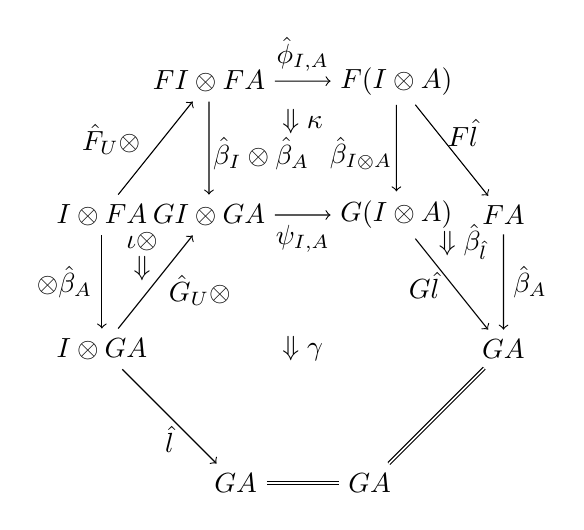
\begin{tikzpicture}[scale=1.7]
\node (llb) at (0,1) {$I \otimes GA$};
\node (llt) at (0,2) {$I \otimes FA$};
\node (bbl) at (1,0) {$GA$};
\node (bml) at (0.8,2) {$GI \otimes GA$};
\node (tl) at (0.8,3) {$FI \otimes FA$};
\node (bbr) at (2,0) {$GA$};
\node (bmr) at (2.2,2) {$G(I \otimes A)$};
\node (tr) at (2.2,3) {$F(I \otimes A)$};
\node (brr) at (3,1) {$GA$};
\node (trr) at (3,2) {$FA$};
\draw[->] (llb) to node [below]{$\hat{l}$} (bbl);
\draw[->] (llt) to node [left]{$\id \otimes \hat{\beta}_A$} (llb);
\draw[->] (llt) to node [above,xshift=-16pt,yshift=-6pt]{${\hat{F}_U} \otimes \id$} (tl);
\draw[->] (llb) to node [below, xshift=16,yshift=6]{$ \hat{G}_U \otimes \id$} (bml);
\draw[->] (tl) to node [above]{$\hat{\phi}_{I,A}$} (tr);
\draw[->] (bml) to node [below] {$\psi_{I,A}$} (bmr);
\draw[double] (bbl) to (bbr);
\draw[double] (bbr) to (brr);
\draw[->] (tr) to node [above,xshift=4, yshift=-2]{$F\hat{l}$} (trr);
\draw[->] (bmr) to node [below,xshift=-10,yshift=8] {$G \hat{l}$} (brr);
\draw[->] (trr) to node [right]{$\hat{\beta}_A$} (brr);
\draw[->] (tl) to node [right,xshift=-2,yshift=-2]{$\hat{\beta}_I \otimes \hat{\beta}_A$} (bml);
\draw[->] (tr) to node [left,xshift=2,yshift=-2]{$\hat{\beta}_{I \otimes A}$} (bmr);
\node at (1.5, 2.7) {$\Downarrow \kappa$};
\node at (0.3, 1.6) {$\Downarrow$};
\node at (0.3, 1.8) {$\iota \otimes \id$};
\node at (2.7,1.8) {$\Downarrow \hat{\beta}_{\hat{l}}$};
\node at (1.5, 1) {$\Downarrow \gamma$};
\end{tikzpicture}
\end{aligned}
\end{equation}

All individual 2-cells are $\theta$-isomorphisms, by Lemmas ~\ref{thm:comp-ten} and ~\ref{thm:theta-nat}. The equality follows by uniqueness of $\theta$-isomorphisms.
\end{proof}

\begin{lem}\label{lem:brtran}
Let $\beta: (F, \phi) \rightarrow (G,\psi)$ be a {\bf braided monoidal vertical transformation}. The image of $\beta$ under $\mathcal{H}$, $\hat{\beta}: (F, \phi) \rightarrow (G,\psi)$ is a braided monoidal pseudonatural adjoint equivalence.
\end{lem}

\begin{proof}
We need to verify that axiom (BTA1) of ~\cite{mccrudden:bal-coalgb} holds, which is given below.

\begin{equation}
\begin{aligned}
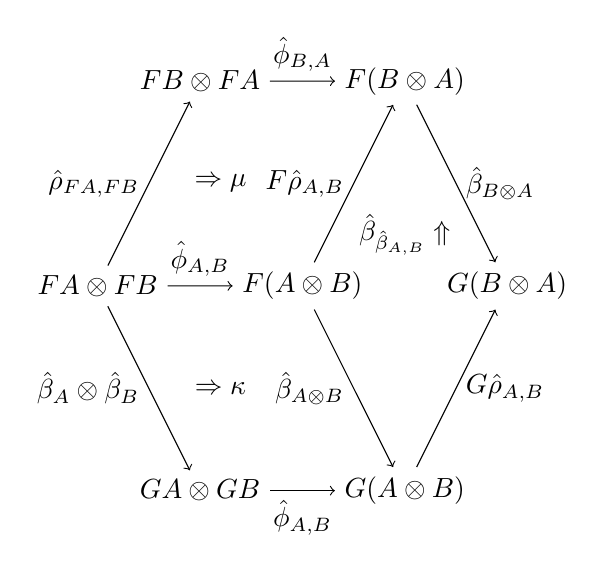
\begin{tikzpicture}[scale=1.3]
\node (tl) at (1,4) {$FB \otimes FA$};
\node (tr) at (3,4) {$F(B \otimes A)$};
\node (ml) at (0,2) {$FA \otimes FB$};
\node (mm) at (2,2) {$F(A \otimes B)$};
\node (mr) at (4,2) {$G(B \otimes A)$};
\node (bl) at (1,0) {$GA \otimes GB$};
\node (br) at (3,0) {$G(A \otimes B)$};
\draw[->] (tl) to node [above] {$\hat{\phi}_{B,A}$} (tr);
\draw[->] (ml) to node [left] {$\hat{\rho}_{FA,FB}$} (tl);
\draw[->] (ml) to node [above] {$\hat{\phi}_{A,B}$} (mm);
\draw[->] (mm) to node [left] {$F\hat{\rho}_{A,B}$} (tr);
\draw[->] (tr) to node [right] {$\hat{\beta}_{B\otimes A}$} (mr);
\draw[->] (mm) to node [left] {$\hat{\beta}_{A\otimes B}$} (br);
\draw[->] (br) to node [right] {$G\hat{\rho}_{A,B}$} (mr);
\draw[->] (bl) to node [below] {$\hat{\phi}_{A,B}$} (br);
\draw[->] (ml) to node [left] {$\hat{\beta}_A \otimes \hat{\beta}_B$} (bl);
\node at (1.2,3) {$\Rightarrow \mu$};
\node at (1.2,1) {$\Rightarrow \kappa$};
\node at (3,2.5) {$\hat{\beta}_{\hat{\beta}_{A,B}}\Uparrow$};
\end{tikzpicture}
\end{aligned}
\hspace{0.25cm}
=
\hspace{0.25cm}
\begin{aligned}
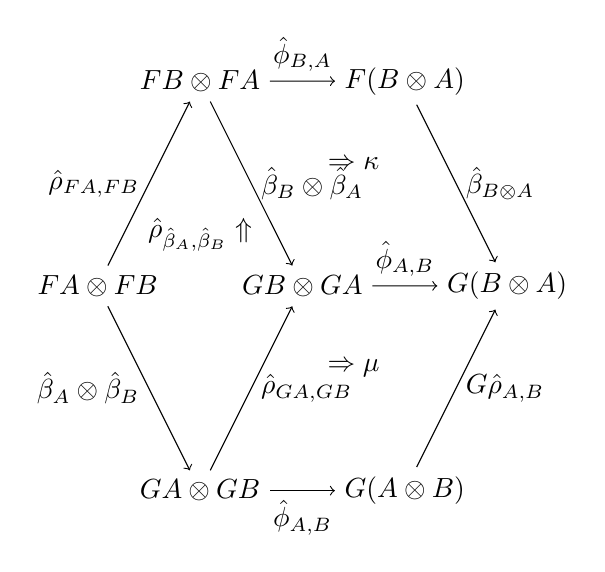
\begin{tikzpicture}[scale=1.3]
\node (tl) at (1,4) {$FB \otimes FA$};
\node (tr) at (3,4) {$F(B \otimes A)$};
\node (ml) at (0,2) {$FA \otimes FB$};
\node (mm) at (2,2) {$GB \otimes GA$};
\node (mr) at (4,2) {$G(B \otimes A)$};
\node (bl) at (1,0) {$GA \otimes GB$};
\node (br) at (3,0) {$G(A \otimes B)$};
\draw[->] (tl) to node [above] {$\hat{\phi}_{B,A}$} (tr);
\draw[->] (ml) to node [left] {$\hat{\rho}_{FA,FB}$} (tl);
\draw[->] (tl) to node [right] {$\hat{\beta}_B \otimes \hat{\beta}_A$} (mm);
\draw[->] (mm) to node [above] {$\hat{\phi}_{A,B}$} (mr);
\draw[->] (tr) to node [right] {$\hat{\beta}_{B\otimes A}$} (mr);
\draw[->] (bl) to node [right] {$\hat{\rho}_{GA,GB}$} (mm);
\draw[->] (br) to node [right] {$G\hat{\rho}_{A,B}$} (mr);
\draw[->] (bl) to node [below] {$\hat{\phi}_{A,B}$} (br);
\draw[->] (ml) to node [left] {$\hat{\beta}_A \otimes \hat{\beta}_B$} (bl);
\node at (1,2.5) {$\hat{\rho}_{\hat{\beta}_A,\hat{\beta}_B} \Uparrow $};
\node at (2.5,3.2) {$\Rightarrow \kappa$};
\node at (2.5,1.2) {$\Rightarrow \mu$};
\end{tikzpicture}
\end{aligned}
\end{equation} 

All individual 2-cells are $\theta$-isomorphisms, either by Lemma \ref{thm:theta-nat} or by definition. The equality follows from Lemma \ref{lem:equal}.
\end{proof}

\begin{cor}\label{cor:symtran}
Let $\beta: (F, \phi) \rightarrow (G,\psi)$ be a {\bf symmetric monoidal vertical transformation}. The image of $\beta$ under $\mathcal{H}$, $\hat{\beta}: (F, \phi) \rightarrow (G,\psi)$, is a symmetric monoidal pseudonatural adjoint equivalence.
\end{cor}

\begin{proof}
Symmetric monoidal adjoint equivalences are simply braided adjoint equivalences between symmetric monoidal pseudofunctors. 
\end{proof}

This brings us to the proof of our theorem.

\begin{proof}[Proof of Theorem \ref{thm:trifunctor2}]
Combining Lemmas \ref{lem:monfun}, \ref{lem:brfun},  \ref{lem:symfun}, \ref{lem:montran}, \ref{lem:brtran} and Corollary \ref{cor:symtran} gives the required result.
\end{proof}
